%Slide 03. Fraud Analysis and Detection
%Frauds: definition and types
% Fraud detection and prevention
% Big data and analytics
% Fraud analytics process model
\chapter{Frauds: definition and types}
\section{What is a fraud?}
    \textit{Wrongful or criminal deception intended to result in financial or personal gain}\\
    \textit{Fraud is an uncommon, well-considered, imperceptibly concealed, time-evolving and often carefully organized crime which appears in many types of forms}\\
    The two definitions toghether explain well what a fraud is. The second expecially gives us the fraud's characteristics.\\
    A fraud is:
    \begin{itemize}
        \item a \textbf{social phenomenon}
        \item \textbf{Uncommon:} usually the percentace of frauds is very small. Only a minority of cases concerns frauds, and only a limited number of them will be \textbf{known} to concern fraud.\\
        This makes them difficult to \textbf{be detected}, because fraudulent cases are covered by legitimate ones, and makes difficult to \textbf{learn from historical cases}, because of the small number of available samples.
        \item \textbf{Well considered and imperceptibly concealed:} fraudsters try to remain \textit{unnoticed and covered}, they blend in\footnote{mimetizzano} frauds by not-behaving differently from non-fraudsters. Fraudsters \textbf{hide} very well by well-considering and planning how to precisely commit fraud
        \item \textbf{Time-evolving:} since fraud detection systems improve and learn by example, fraudsters adapt and refine their methods to remain undetected. Fraudsters techniques evolve in time along with or better ahead of fraud detection mechanisms. This is an adversarial situation in which usually the fraudster is always ahead. Each security solution has a cost which can be a waste if the fraudster is able to break it in days.\\
        Not only frauds change, but also the legitimate behavior of the users. Also this must be followed in time, this is called concept drift: legitimate behavior of models changes in time.
        \item \textbf{Carefully organized crime:} they're not usually composed of a single operation, and fraudsters belong to a complex and organized structure. The entire cybercrime group (context) after a fraud must be investigated.
    \end{itemize}
\section{Cybercriminal ecosystem}
    \begin{figure}[!ht]
        \subfigure{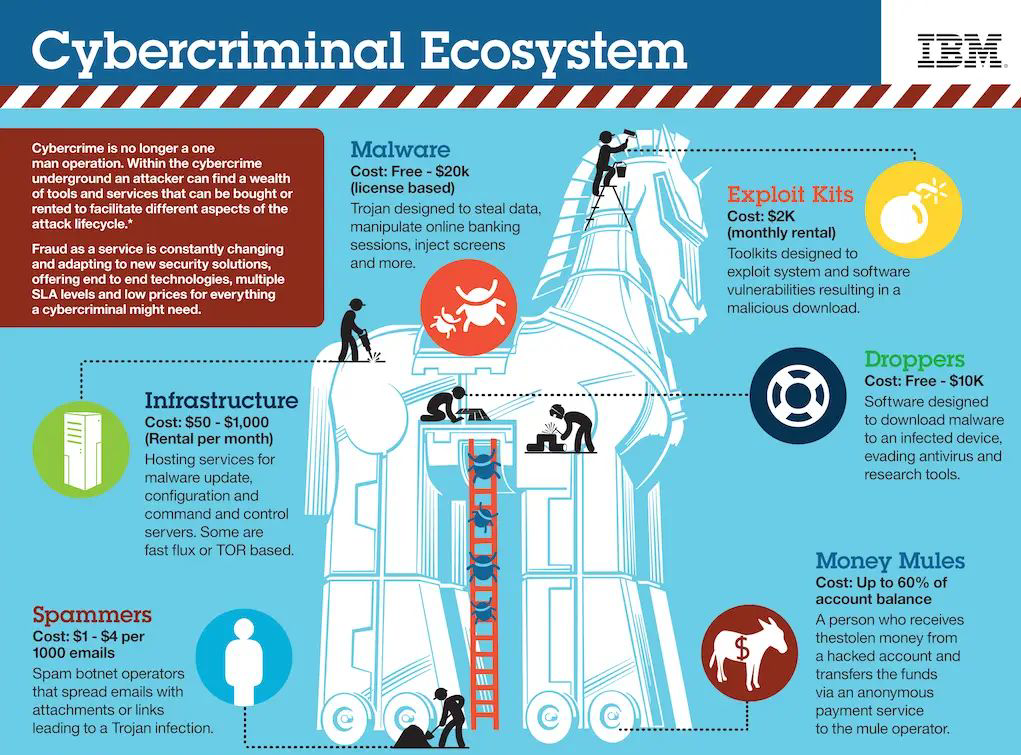
\includegraphics[width=0.45\linewidth]{eco.png}}
        \subfigure{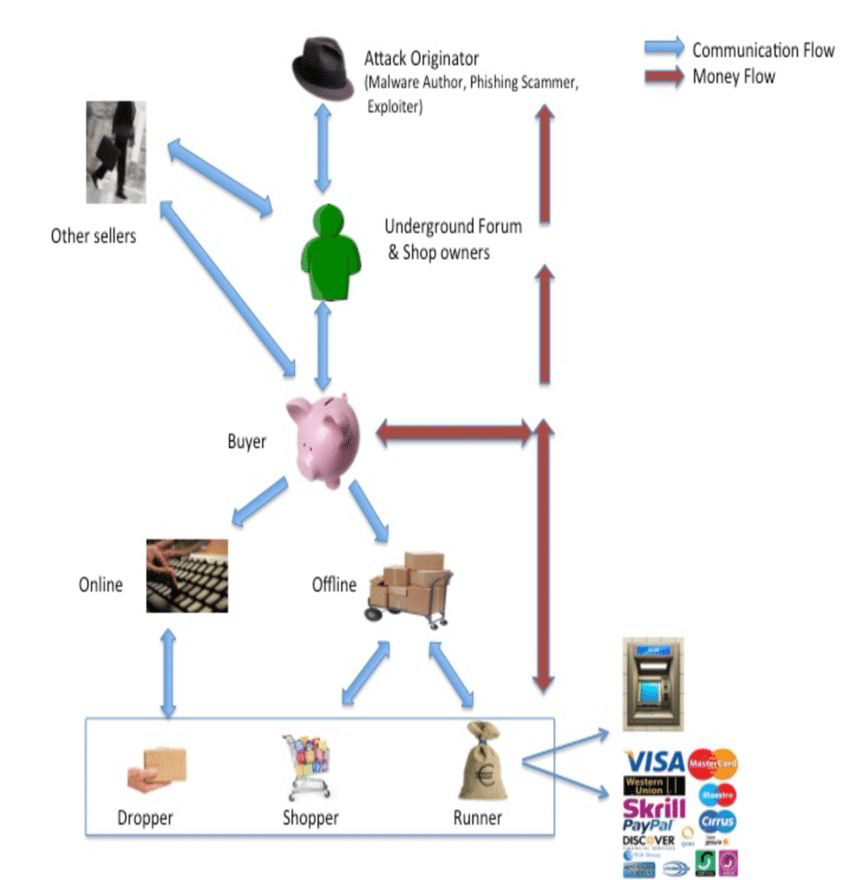
\includegraphics[width=0.45\linewidth]{eco2.png}}
    \end{figure}
    \begin{itemize}
        \item Some groups are specialized in creating malwares
        \item Some in providing infrastructures to perform money laundering
        \item Others to perform financial crimes
        \item Others spamming, phishing 
        \item Others exploiting 
    \end{itemize}
    Every single time we think about a financial fraud, what we see is just the last part of an entire interaction between criminals in the entire ecosystem.\\ 
    A buyer usually isn't able to perform cyber-crimes, he just interacts with criminals trough forums to pay for their services, which put toghether form a crime.
\section{Why do people commit frauds?}
    \begin{figure}[!ht]
        \centering
        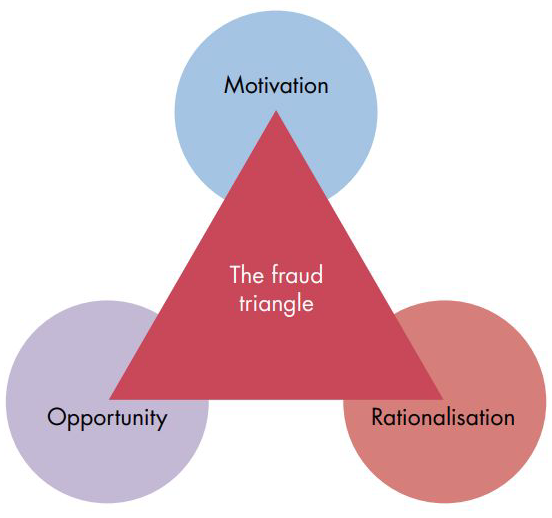
\includegraphics[width=0.45\linewidth]{triangle.png}
    \end{figure}
    The \textit{basic driver} for committing fraud is the \textbf{potential monetary gain or benefit}. The fraud triangle is a general model that tries to define which are the drivers for fraudsters:
    \begin{itemize}
        \item Motivation: usually the need to escape from a tragic situation, or just greed 
        \item Opportunity: the fraudsters know that a system has low security or they know someone from the inside that knows about some vulnerability to exploit 
        \item Rationalisation: usually they perform frauds when they think that what they're doing is \textit{not so bad}
    \end{itemize}
    Fraud detection and prevention systems aim to reduce as much as possible the opportunities for attackers, making attacks non-convenient.
\section{Fraud categories}
    \begin{itemize}
        \item \textbf{Banking and credit card frauds:} Unauthorized taking of another's credit. They happen in two different ways:
        \begin{itemize}
            \item \textbf{Application fraud:} the target is the company, which is convinced to release a credit card under a fake identity. Then, fraudsters spend as much as possible in a short space of time.
            \item \textbf{Behavioral fraud:} the target is a user, details of legitimate cards are obtained fraudulently by stealing credentials.
        \end{itemize}
        \item \textbf{Insurance Frauds:} Related to any type of insurance
        \begin{itemize}
            \item Selling nonexistent policies
            \item Buying policies to get paid from fake incidents
        \end{itemize}
        \item \textbf{Corruption:} The misuse of entrusted power for private gain
        \item \textbf{Counterfeit:} An imitation intended to be passed off deceptively as genuine. Tipically concerns valuable objects like credit cards, IDs, popular products, money \dots
        \item \textbf{Product warranty fraud:} A fraud that tries to exploit the warranty of a product
        \item \textbf{Healthcare fraud:} Filling of dishonest healthcare claims to make profit. Common in the US.
        \item \textbf{Telecommunications fraud:} Theft or use of telecommunication services to commit other forms of fraud
        \item \textbf{Money laundering:} Taking the proceeds of criminal activity and making them appear legal. Usually one of the most effective and efficient crimes 
        \item \textbf{Click fraud:} Illegal clicks on a website's advertisements to increase the payable number of clicks
        \item \textbf{Identity theft:} Obtaining the personal or financial information of another person for the purpose of assuming that person's identity to make transactions or purchases
        \item \textbf{Tax Evasion:} Illegal act or practice of failing to pay taxes that are owed 
        \item \textbf{Plagiarism:} Steal and pass off the ideas or words of another as own
    \end{itemize}
    \subsection{Social Engineering}
        It is one of the main vectors to perform frauds. Attackers use human interaction to obtain or compromise information by psychologically manipulating a person into knowlingly or unknowingly giving up information.\\
        It essentially means \textit{hacking} into a person to steal valuable information from many sources. It consistently works, while technology vulnerabilities are hardened and solved.\\
        The attackers usually address the weakest element of the system, which is most of the times the user. There is no patch for human stupidity.
        \begin{figure}[!ht]
            \centering
            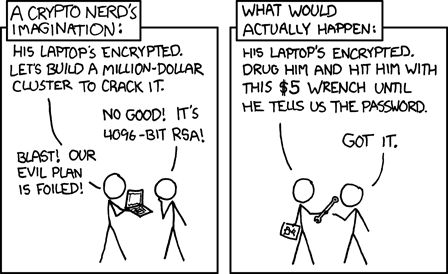
\includegraphics[width=0.45\linewidth]{memes.png}
        \end{figure}
        \subsection{Famous social engineering cases}
            \begin{itemize}
                \item \textbf{Kevin Mitnick}
                \item \textbf{Frank Abagnale}
            \end{itemize}
        \subsubsection{Phishing}
            Is the fraudulent process of attempting to acquire sensitive information by masquerading as a trustworthy entity in an electronic communication.
        \subsubsection{The Nigerian Prince Scam}       
            Email requesting the victim to help a Nigerian Prince into retrieving the money from an account. Part of money laundering where the victim is the only one persecutable.
        \subsubsection{Vishing}
            To steal or change someone credentials by faking to be someone else and convincing their keeper
        \subsubsection{Getting dressed}
            People dressed in certain ways are able to convince other people surrounding them to be someone which is allowed to do something like asking money from the cashier faking to be a bank guard.
    \subsection{Frauds Impact}
        Frauds is often mistakenly considered to be a victimless crime, but actually it has an impact:
        \begin{itemize}
            \item A typical organizations loses 5\% of its revenues to fraud each year
            \item The total cost of insurance fraud in the USA is estimated to be more than \$40 billion per year 
            \item Fraud costs the United Kingdom £73 billion a year
            \item Credit card companies lose approximately 7 cents per every hundred dollars of transactions due to fraud
        \end{itemize}
        There is a need to invest into \textbf{up-to-date defense infrastructures}
\section{Anti-Fraud Strategy}
    Advanced anti fraud mechanisms:
    \begin{itemize}
        \item Reduce losses due to fraud
        \begin{itemize}
            \item Prevented \& Detected
            \item Fraudsters tend to look for the easy way and will look for easier opportunities 
        \end{itemize}
    \end{itemize}
    We call:
    \begin{itemize}
        \item \textbf{Fraud detection:} the process to recognize or discover frauds once they happen (ex-post approach)
        \item \textbf{Fraud prevention:} the set of techniques used to avoid or reduce frauds (ex-ante approach)
    \end{itemize}
    \subsection{Example: Banking Fraud}
        \begin{figure}[!ht]
            \centering
            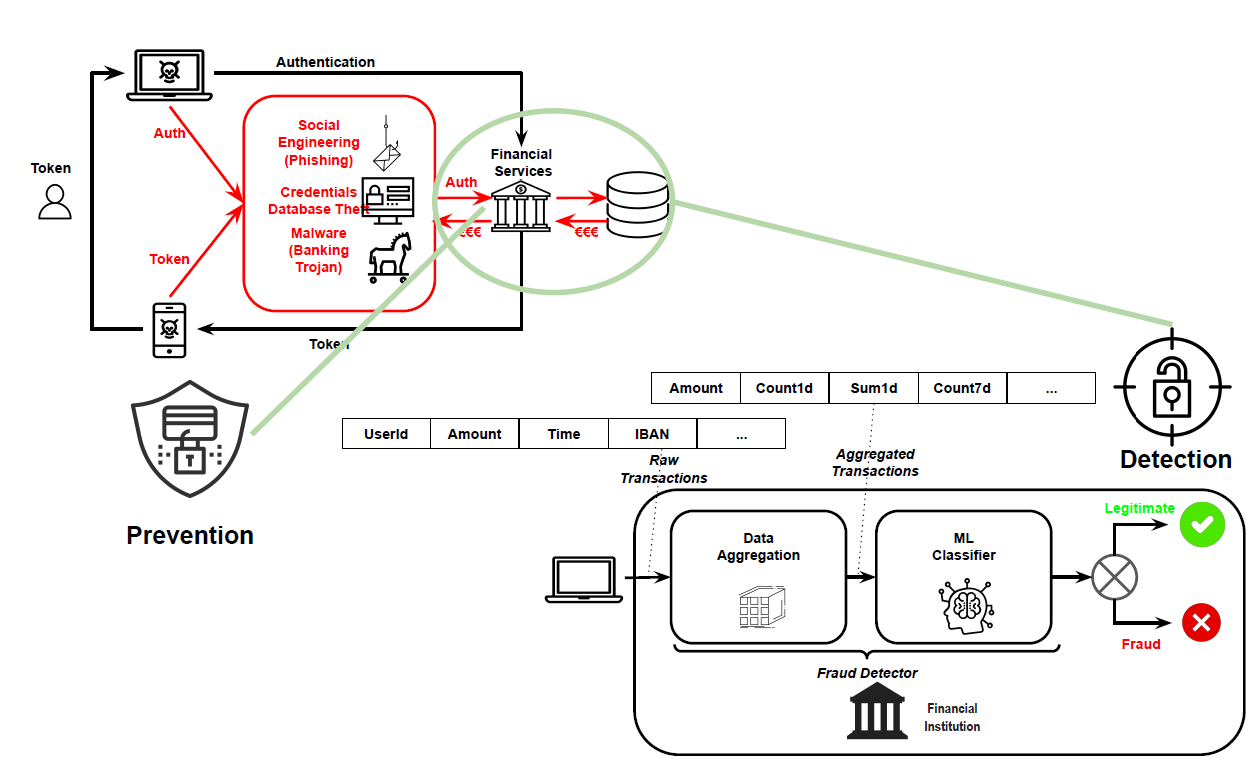
\includegraphics[width=0.45\linewidth]{bank_example.png}
        \end{figure}
        The system must be defended on the financial services side, because phone and laptop are compromised.\\ 
        The system tries to prevent frauds before they are executed and detect frauds after. These kind of systems are based on Machine Learning usually, automatically analizing data in order to understand what is legitimate and what is not.
    \subsection{Fraud Detection and Prevention}
        They are \textbf{complementary} but not independent:
        \begin{itemize}
            \item Fraudsters adapt to the prevention mechanism changing their behavior, this impacts the detection mechanism.
            \item This also happens for the detection mechanism, impacting the prevention mechanism.
        \end{itemize}
        So what happens is that both are updated in order to impact in the good sense the other mechanism.
\newpage
    \subsection{Fraud Detection approach}
        \begin{figure}[!ht]
            \centering
            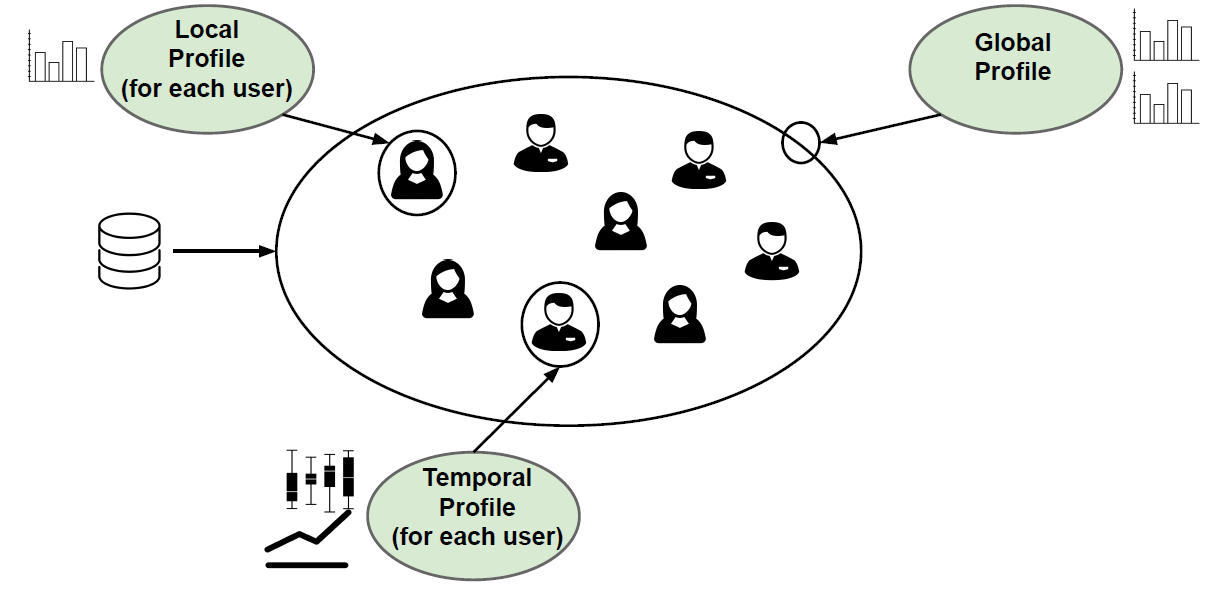
\includegraphics[width=0.45\linewidth]{fraudanalysis.png}
        \end{figure}
        Data are analised by:
        \begin{itemize}
            \item A local perspective: local profile characterizes each user's spending pattern to evaluate the anomaly of new transaction
            \item A global perspective: global profile characterizes \textit{classes} of spending patterns and mitigate the undertraining problem 
            \item Temporal Profile deals with frauds that exploit the repetition of legitimate looking transactions over time 
        \end{itemize}
        In the end a score is computed for each single transaction, scoring the risk of them to be frauds. At the end of the day, all of the fraudulent-checked transactions are personally verified by real people.\\
        Consider that this has a cost. False positive can also make the organization to lose clients.
    \subsection{Fraud prevention mechanism}
        All mechanism put in place to implement strong customer authentication: a European regulatory requirement to reduce fraud and make online payments more secure.\\
        Strong Customer Authentication requires to use at least two out of the following elements:
        \begin{itemize}
            \item Something the customer knows: such as a password
            \item Something the customer has: phone or hardware token 
            \item Something the customer is: such as fingerprint
        \end{itemize}
        \subsubsection{Classic technologies}
            One time password generators used to generate part of the code required to online payments by the use of the other part, smart cards with private keys were able to generate a password based on the user's card.\\
            Static OTP lists were a list of codes usable to perform some operations.
        \subsubsection{Modern Technology}
            Nowadays software implement the same functionalities of password generators.
        \subsubsection{Attackers adapt to it}
            \begin{itemize}
                \item Sim swapping attack: to obtain codes usually the user receives a PIN over sms. Attackers contact phone carriers to make them give a new SIM card by pretending to be you.
                \item Another attack was a social engineering attack to steal banking credentials, perform a transaction without having the code, calling you by faking to be your bank to tell you to provide the token to block a transaction while actually performing it.
            \end{itemize}
        